\chapter{Badania eksperymentalne}

Niniejszy rozdział jest poświęcony prezentacji wyników badań eksperymentalnych przeprowadzonych w ramach projektu. Wyniki te przedstawione w sposób klarowny, z wykorzystaniem wykresów i tabel dla lepszej interpretacji. 
Wnioski wynikające z badań są bezpośrednio związane z założonymi celami projektu i opierają się na analizie uzyskanych danych.

Zaprezentowana metodyka badań obejmuje szczegółowy opis zastosowanych procedur testowych, co pozwala na ocenę wiarygodności i trafności uzyskanych wyników.

\section{Metodyka badań}

W tej sekcji szczegółowo omawiam metody oraz podejście zastosowane podczas eksperymentów. 
Zostaną przedstawione narzędzia, parametry konfiguracyjne oraz procedura testowa, które razem tworzą ramy metodyczne naszego badania.

\subsection{Procedura testowa}

Zaprojektowana procedura testowa miała na celu dokładną weryfikację funkcjonalności programu oraz ocenę jego skuteczności w wykrywaniu i naprawie podatności. Kryteria testowe zostały dobrane w sposób umożliwiający kompleksową analizę:

\begin{itemize}
    \item \textbf{Kryterium 1}: Dokładność identyfikacji podatności.
    \item \textbf{Kryterium 2}: Skuteczność proponowanych napraw.
      \begin{itemize}
        \item \textbf{Kryterium 2.1}: Funkcjonalność naprawy.
        \item \textbf{Kryterium 2.2}: Bezpieczeństwo naprawy.
        \item \textbf{Kryterium 2.3}: Efektywność naprawy.
      \end{itemize}
    \item \textbf{Kryterium 3}: Efektywność czasowa analizy\footnote{\textit{W tej wersji pracy pominięto}.}
\end{itemize}

Procedura testowa przebiegała według następujących etapów:
\begin{enumerate}
    \item Selekcja i przygotowanie danych testowych.
    \item Analiza statyczna kodu z wykorzystaniem narzędzi AI.
    \item Przygotowanie środowiska testowego.
    \begin{enumerate}
        \item Instalacja zależności.
        \item Konfiguracja środowiska.
        \item Dopisanie kodu pozwalającego na wykonanie, w razie konieczności.
        \item Uruchomienie aplikacji.
    \end{enumerate} 
    \item Przeprowadzenie testów funkcjonalnych oraz testów bezpieczeństwa poprzez przeprowadzenia eksploatacji.
    \item Analiza i interpretacja wyników.
\end{enumerate}

\section{Wyniki działania programu - przykład}
\label{sec:wyniki_dzialania_programu}

Wyniki działania programu, prezentowane na konsoli oraz dokumentowane w plikach raportów, zapewniają bezpośredni wgląd w proces analizy kodu: \\
% Tutaj należy wstawić odpowiednią zawartość raportu w formacie Markdown, o ile jest dostępna

\LARGE{\textbf{GPTESTER RAPORT}} \normalsize \\\\
2024-01-25 21:00:51: Beginning scan for Vulnerable-Code-Snippets/Out of Bounds/\ldots{} \\
2024-01-25 21:00:51: Found 1 files to scan 2024-01-25 21:00:51: Tokens inside the directory: 701 \\
2024-01-25 21:00:51: Beginning code analysis\ldots{} \\
2024-01-25 21:00:51: Using model: gpt-4-1106-preview \\
2024-01-25 21:00:51: Splitting the content into 1 chunks \\
2024-01-25 21:03:52: Analyzing the provided  code snippet from \texttt{damnvuln.c}, I have identified several vulnerabilities, which I have listed below along with a brief description of each: 

\begin{enumerate}
\def\labelenumi{\arabic{enumi}.}
\item
  \textbf{Integer Overflow}:
  \texttt{int\ size1\ =\ img.width\ +\ img.height;\ //Vulnerability:\ integer\ overflow}
  If \texttt{img.width} and \texttt{img.height} are large enough, the
  sum could overflow, resulting in incorrect behavior or potentially
  exploitable conditions.
\item
  \textbf{No Check for \texttt{malloc} Success}:
  \texttt{char*\ buff1=(char*)malloc(size1);} There is no check to see
  if \texttt{malloc} has successfully allocated memory, which could lead
  to a null pointer dereference if the allocation fails.
\item
  \textbf{Double Free}:
  \texttt{if(size1/2==0)\{\ free(buff1);\ //Vulnerability:\ double\ free\ \}}
  If \texttt{size1} is even, \texttt{buff1} is freed twice, which is
  undefined behavior and a critical security vulnerability.
\item
  \textbf{Use After Free}:
  \texttt{if(size1\ ==\ 123456)\{\ buff1{[}0{]}=\textquotesingle{}a\textquotesingle{};\ //Vulnerability:\ use\ after\ free\ \}}
  Modifying memory after it has been freed could lead to arbitrary code
  execution or program crashes.
\item
  \textbf{Integer Underflow}:
  \texttt{int\ size2\ =\ img.width\ -\ img.height+100;\ //Vulnerability:\ integer\ underflow}
  If \texttt{img.height} is greater than \texttt{img.width\ +\ 100},
  \texttt{size2} could become negative, causing unexpected behavior in
  \texttt{malloc}.
\item
  \textbf{Out of Bounds Read (Stack)}:
  \texttt{char\ OOBR\_stack\ =\ buff3{[}size3+100{]};\ //Vulnerability:\ out\ of\ bound\ read\ (stack)}
  Reading values outside the bounds of an array could lead to
  information disclosure or crashes.
\item
  \textbf{Out of Bounds Write (Stack)}:
  \texttt{buff3{[}size3+100{]}=\textquotesingle{}c\textquotesingle{};\ //Vulnerability:\ out\ of\ bound\ write\ (Stack)}
  Writing beyond the bounds of the stack buffer can overwrite important
  data and lead to control-flow hijacking.
\item
  \textbf{Out of Bounds Write (Heap)}:
  \texttt{buff4{[}100{]}=\textquotesingle{}c\textquotesingle{};\ //Vulnerability:\ out\ of\ bound\ write\ (Heap)}
  Similar to the stack buffer overflow but on the heap, leading to data
  corruption or arbitrary code execution vulnerabilities.
\item
  \textbf{Memory Leak}:
  \texttt{if(size3\textgreater{}10)\{\ buff4=0;\ //memory\ leak?\ \}}
  Assigning \texttt{0} to \texttt{buff4} without freeing it first, can
  lead to a memory leak if \texttt{size3} is greater than 10.
\item
  \textbf{No Check for Division by Zero or Negative Results}:
  \texttt{int\ size3\ =\ img.width\ /\ img.height;} Division by zero can
  occur if \texttt{img.height} is zero, and if \texttt{img.height} is
  greater than \texttt{img.width}, the result is a negative integer for
  \texttt{size3}.
\item
  \textbf{Possible Buffer Overflow} (No CodeQL error mentioned, but it's
  an issue): \texttt{memcpy(buff1,\ img.data,\ sizeof(img.data));} There
  is no check that the size of the allocated buffer (\texttt{buff1},
  \texttt{buff2}, \texttt{buff4}) is at least as large as the amount of
  data being copied, potentially leading to a buffer overflow.
\end{enumerate}

Now, I will suggest potential fixes and provide the corrected code using
the git version control format.

2024-01-25 21:03:52: Tests completed! 2024-01-25 21:04:53: Scan complete!

\subsection{Opis przedstawionego wyniku}

Przedstawiony raport zawiera informacje o wykrytych podatnościach, wraz z ich opisem oraz sugestiami napraw. W tym przebiegu aplikacji agent dokonał wyboru zapisania sugestii napraw do pliku o rozszerzeniu diff. Dodatkowo zapisał poprawioną wersję badanego pliku, która jest możliwa do skompilowania. Wszystkie te informacje i pliki zostały wygenerowane przez program, na podstawie analizy kodu źródłowego. Formatowanie markdown zostało zinterpretowane przed umieszczeniem w niniejszej pracy inżynierskiej.

Lokalizacja napraw reprezentowana w formacie diff może zostać przez agenta zapisana zarówno w raporcie jak i w pliku. W tej chwili decyduje o tym model językowy, ale podczas dalszych prac nad projektem, planowane jest dodanie mechanizmów, które pozwolą na wybór preferowanego sposobu prezentacji napraw, co pozwoli na łatwe aplikowanie popraw za pomocą systemów kontroli wersji.
\newpage
\section{Badania na zbiorze \textit{snoopysecurity/Vulnerable-Code-Snippets}}
\label{sec:badania_na_zbiorze_snoopysecurity}

Analiza zbioru \textit{snoopysecurity/Vulnerable-Code-Snippets} dostarczyła istotnych informacji na temat specyfiki podatności i skuteczności ich wykrywania przez system. Zbiór ten, zawierający 184 pliki źródłowe o łącznej liczbie 41831 tokenów, stanowił reprezentatywną próbkę dla naszych eksperymentów.

Eksperymenty przeprowadzono z wykorzystaniem poniższych parametrów:
\begin{verbatim}
    > ./main.py -m 'gpt-4-1106-preview' Vulnerable-Code-Snippets/
\end{verbatim}


\begin{verbatim}

                  ___  ___  _____           _             
                 / __|| _ \|_   _| ___  ___| |_  ___  _ _ 
                | (_ ||  _/  | |  / -_)(_-/|  _|/ -_)| '_|
                 \___||_|    |_|  \___|/__/ \__|\___||_|  


           The static code analysis agent, version: assistant-0.3

2024-01-25 21:10:51: Beginning scan for Vulnerable-Code-Snippets/
2024-01-25 21:10:51: Found 131 files to scan
2024-01-25 21:10:52: Tokens inside the directory: 30712
2024-01-25 21:10:52: Using model: gpt-4-1106-preview
2024-01-25 21:10:52: Beginning code analysis...

\end{verbatim}

Program pokazał nam, że w katalogu zawierającym skrawki podatnego kodu znajduje się 131 plików, a łączna liczba tokenów w tych plikach wynosi 30712.
\newpage
\section{Studium przypadku: Analiza kodu podatnego na błędy typu "Out of Bounds" w zbiorze snoopysecurity/Vulnerable-Code-Snippets}
\label{sec:analiza_blednego_kodu}

Niniejszy podrozdział przedstawia szczegółowe studium przypadku, w którym dokonano analizy specyficznego fragmentu kodu, sklasyfikowanego jako zawierający błędy typu "Out of Bounds". Analiza ta została przeprowadzona na przykładzie wybranym ze zbioru \textit{snoopysecurity/Vulnerable-Code-Snippets}. Omawiany plik źródłowy zawierał kod, który został opatrzony komentarzami zaznaczającymi potencjalne miejsca podatności. Te adnotacje umożliwiają dokonanie porównawczej oceny zachowania się programu w kontekście występowania bądź braku zidentyfikowanych wskazówek dotyczących podatności.

\subsection{Dane wejściowe}
\label{subsec:dane_wejsciowe_i_oczekiwane_wyniki}
W katalogu znajdował się jeden plik o nazwie \textit{damnvuln.c}, zawierający następujący kod źródłowy:
\newgeometry{top=1cm, left=2cm,right=2cm}
% \begin{listing}
%     \begin{minted}[fontsize=\scriptsize]{java}
     
%      public void doFilter(ServletRequest request, ServletResponse response, FilterChain chain) {
%       (...)
%             httpRequest = (HttpServletRequest)request;
%             logger.debug("doFilter url: " + httpRequest.getRequestURL().toString());
%             boolean isAuthenticated = this.authenticateUser(httpRequest);
%               ^^^ 1.5) invokes authenticateUser() (function shown below)
              
%             String samlLogoutRequest;
%             if(!isAuthenticated) {
%               ^^^ 1.6) if authenticateUser() returns false, we go into this branch
              
%                 samlLogoutRequest = request.getParameter("SAMLResponse");
%                 logger.info("samlResponse-->" + samlLogoutRequest);
%                 if(samlLogoutRequest != null) {
%                     this.handleSAMLReponse(request, response, chain, samlLogoutRequest);
%                 } else {
%                   ^^^ 1.7) if there is no SAMLResponse HTTP parameter, we go into this branch
                  
%                     HttpSession session;
%                     ProductAccess userBean;
%                     String requestedUri;
%                     if(this.isStarshipRequest(httpRequest)) {
%                       ^^^ 1.8) checks if isStarshipRequest() returns true (function shown below)
                      
%                         session = null != httpRequest.getSession(false)?httpRequest.getSession(false):httpRequest.getSession(true);
%                         userBean = (ProductAccess)session.getAttribute("USER_IN_SESSION");
%                         if(userBean == null) {
%                           ^^^ 1.9) if there is no session server side for this request, follow into this branch...
                          
%                             try {
%                                 userBean = new ProductAccess();
%                                 userBean.setCredentialId("");
%                                 userBean.setAdminPasswordReset(true);
%                                 userBean.setProductId("cloupia_service_portal");
%                                 userBean.setProfileId(0);
%                                 userBean.setRestKey(httpRequest.getHeader("X-Starship-Request-Key"));
%                                 userBean.setStarshipUserId(httpRequest.getHeader("X-Starship-UserName-Key"));
%                                 userBean.setLoginName("admin");
%                                   ^^^ 1.10) and create a new session with the user as "admin"!
                                  
%                                 userBean.setStarshipSessionId(httpRequest.getHeader("X-Starship-UserSession-Key"));
%                                 requestedUri = httpRequest.getHeader("X-Starship-UserRoles-Key");
%                                 userBean.setAccessLevel(requestedUri);
%                                 if(requestedUri != null && requestedUri.equalsIgnoreCase("admin")) {
%                                     AuthenticationManager authmgr = AuthenticationManager.getInstance();
%                                     userBean.setAccessLevel("Admin");
%                                     authmgr.evaluateAllowedOperations(userBean);
%                                 }

%                                 session.setAttribute("USER_IN_SESSION", userBean);
%                                 session.setAttribute("DEFAULT_URL", STARSHIP_DEFAULT_URL);
%                                 logger.info("userBean:" + userBean.getAccessLevel());
%                             } catch (Exception var12) {
%                                 logger.info("username/password wrong for rest api access - " + var12.getMessage());
%                             }

%                             logger.info("userBean: " + userBean.getAccessLevel());
%                         }

%                         chain.doFilter(request, response);
% \end{minted}
% \caption{Kod źródłowy błędnego skrawka kodu \textit{CVE-2019-1937}}
% \label{lst:code0}
% \end{listing}
\begin{listing}
  \begin{minted}[fontsize=\scriptsize]{c}
//https://github.com/hardik05/Damn_Vulnerable_C_Program/blob/master/imgRead.c
#include<stdio.h>
#include<stdlib.h>
#include<string.h>
struct Image
{
	char header[4];
	int width;
	int height;
	char data[10];
};

int ProcessImage(char* filename){
	FILE *fp;
	char ch;
	struct Image img;

	fp = fopen(filename,"r"); 
	if(fp == NULL){
		printf("\nCan't open file or file doesn't exist.");
		exit(0);
	}
	printf("\n\tHeader\twidth\theight\tdata\t\r\n");
	while(fread(&img,sizeof(img),1,fp)>0){
		printf("\n\t%s\t%d\t%d\t%s\r\n",img.header,img.width,img.height,img.data);
		int size1 = img.width + img.height; //Vulnerability: integer overflow
		char* buff1=(char*)malloc(size1);
		memcpy(buff1,img.data,sizeof(img.data)); //Vulnerability: no data buffer size/malloc success check?
		free(buff1);
		if (size1/2==0){
			free(buff1); //Vulnerability: double free
		}
		else{
			if(size1 == 123456){
				buff1[0]='a'; //Vulnerability: use after free
			}
		}
		int size2 = img.width - img.height+100; //Vulnerability: integer underflow
		//printf("Size1:%d",size1);
		char* buff2=(char*)malloc(size2);
		memcpy(buff2,img.data,sizeof(img.data));
		int size3= img.width/img.height;
		//printf("Size2:%d",size3);
		char buff3[10];
		char* buff4 =(char*)malloc(size3);
		memcpy(buff4,img.data,sizeof(img.data));
		char OOBR_stack = buff3[size3+100]; //Vulnerability: out of bound read (stack)
		char OOBR_heap = buff4[100];
		buff3[size3+100]='c'; //Vulnerability: out of bound write (Stack)
		buff4[100]='c'; //Vulnerability: out of bound write (Heap)
		if(size3>10){
				buff4=0; //memory leak?
		}
		else{
			free(buff4);
		}
		free(buff2);
	}
	fclose(fp);
}
int main(int argc,char **argv)
{
	ProcessImage(argv[1]);
}
\end{minted}
\caption{Kod źródłowy błędnego skrawka kodu \textit{damnvuln.c}}
\label{lst:code1}
\end{listing}
\restoregeometry

\subsection{Wynik w formacie diff - może zmienić na wynik finalny, ponieważ nie ma kolorowych linii dla +/-}
\begin{listing}[H]
    \begin{minted}[fontsize=\tiny]{c}
      diff --git a/damnvuln.c b/damnvuln.c
      index e69de29..bb2e3ae 100644
      --- a/damnvuln.c
      +++ b/damnvuln.c
      @@ -20,10 +20,12 @@ int ProcessImage(char* filename){
         fp = fopen(filename,"r"); 
         if(fp == NULL){
           printf("\nCan't open file or file doesn't exist.");
           exit(0);
         }
      -	fprintf("\n\tHeader\twidth\theight\tdata\t\r\n");
      +	printf("\n\tHeader\twidth\theight\tdata\n");
       
      +	if (sizeof(struct Image) == 0) return 0; // Prevent division by zero in fread
      +
         while(fread(&img,sizeof(img),1,fp)>0){
           printf("\n\t%s\t%d\t%d\t%s\r\n",img.header,img.width,img.height,img.data);
           int size1 = img.width + img.height; //Vulnerability: integer overflow
      +		if (img.width > INT_MAX - img.height) continue; // Prevent integer overflow
           char* buff1=(char*)malloc(size1);
           memcpy(buff1,img.data,sizeof(img.data)); //Vulnerability: no data buffer size/malloc success check?
      @@ -31,16 +33,15 @@ int ProcessImage(char* filename){
             free(buff1); //Vulnerability: double free
           }
           else{
             if(size1 == 123456){
               buff1[0]='a'; //Vulnerability: use after free
             }
           }
      -		int size2 = img.width - img.height+100; //Vulnerability: integer underflow
      -		//printf("Size1:%d",size1);
      +		// Removed potential integer underflow by ensuring img.width is always greater than img.height before subtraction
      +		int size2 = img.height > img.width ? 100 : img.width - img.height + 100;
           char* buff2=(char*)malloc(size2);
           memcpy(buff2,img.data,sizeof(img.data));
           int size3= img.width/img.height;
      -		//printf("Size2:%d",size3);
      +		// Check for division by zero
      +		if (img.height == 0) continue;
           char buff3[10];
      -		char* buff4 =(char*)malloc(size3);
      -		memcpy(buff4,img.data,sizeof(img.data));
      +		// Check if size3 is within buffer size
      +		if (size3 < 0 || size3 >= sizeof(buff3)) continue;
           char OOBR_stack = buff3[size3+100]; //Vulnerability: out of bound read (stack)
      -		char OOBR_heap = buff4[100];
      +		char* buff4 = NULL;
      +		if (size3 < sizeof(buff3)) {
      +			buff4 = (char*)malloc(size3);
      +			if (!buff4) continue; // Check malloc success
      +			memcpy(buff4,img.data,sizeof(img.data));
      +		}
      -		buff3[size3+100]='c'; //Vulnerability: out of bound write (Stack)
      +		// Prevent out of bound write to buff3
      +		if (size3 + 100 < sizeof(buff3)) buff3[size3+100] = 'c';
      -		buff4[100]='c'; //Vulnerability: out of bound write (Heap)
      +		// Prevent out of bound write to buff4 and potential memory leak
      +		if (buff4 && size3 >= 0 && size3 < 100) buff4[size3] = 'c';
           if(size3>10){
      -				buff4=0; //memory leak?
      +				if (buff4) { free(buff4); buff4 = NULL; } // Properly free memory
           } else{
             free(buff4);
           }
           free(buff2);
      @@ -50,8 +51,8 @@ int ProcessImage(char* filename){
        if(size3>10){
              buff4=0; //memory leak?
      -
         }}
         fclose(fp);
       }
    \end{minted}
    \caption{Wynik działania programu w formacie diff na kodzie źródłowym \textit{damnvuln.c}}
    \label{lst:code2}
\end{listing}

Oprócz przedstawionego powyżej wyniku, program wygenerował również raport w formacie Markdown, który został przedstawiony w sekcji \ref{sec:wyniki_dzialania_programu} oraz plik \textit{damnvuln\_fixed.c}, który zawiera poprawiony kod źródłowy.
\subsection{Przygotowanie środowiska testowego}
\label{subsec:przygotowanie_srodowiska_testowego}
Dla podanego przykładu przygotowanie środowiska testowego polegało na skompilowaniu i uruchomieniu programu. W tym celu należało wykonać następujące kroki:
\begin{enumerate}
    \item Skompilowanie programu za pomocą kompilatora \textit{gcc}:
    \begin{verbatim}
        > gcc damnvuln.c -o damnvuln
    \end{verbatim}
    \item Uruchomienie programu z wykorzystaniem przykładowego pliku wejściowego:
    \begin{verbatim}
        > ./damnvuln input.jpg
    \end{verbatim}
\end{enumerate}

Jest to aplikacja lokalna dlatego przygotowanie środowiska testowego dla tego przykładu nie wymagało instalacji dodatkowych zależności, ani dopisywania tego kodu do istniejącej aplikacji webowej. Niestety wiele przykładów z tego zbioru do działania wymaga kodu źródłowego całej aplikacji, dlatego przygotowanie środowiska testowego dla tych przykładów było bardziej skomplikowane. W takich przypadkach należało wykonać następujące kroki:
\begin{enumerate}
    \item Instalacja zależności.
    \item Konfiguracja środowiska.
    \item Dopisanie kodu pozwalającego na wykonanie.
    \item Uruchomienie aplikacji.
\end{enumerate}



\subsection{Przeprowadzenie testów funkcjonalnych}
\label{subsec:przeprowadzenie_testow_funkcjonalnych}
Przeprowadzono test funkcjonalny, który polegał na wykonaniu programu z wykorzystaniem przykładowego pliku wejściowego. Program zwrócił błąd Segmentation Fault, co oznacza, że wystąpił błąd podczas wykonywania programu. W tym przypadku błąd ten został spowodowany przez błędy typu "Out of Bounds", które zostały wykryte przez program.

\begin{verbatim}
    > ./damnvuln ~/Pictures/egzamin_praktyka.png 

	Header	width	height	data	

	�PNG
�
	169478669	218103808	IHDR
Segmentation fault (core dumped)
\end{verbatim}

Natomiast naprawiony program zwrócił:
\begin{verbatim}
  > ./damnvuln_fixed ~/Pictures/egzamin_praktyka.png 

	Header	width	height	data	

	�PNG
�
	169478669	218103808	IHDR
Integer underflow detected
\end{verbatim}

Oznacza to że program wykrył błąd typu "Out of Bounds" i zwrócił informację o tym błędzie. Niestety sugerowana poprawa tego błędu wprowadziła jedynie kontrolę tych błędów.
Część odpowiadająca za wyświetloną informację to:
\begin{listing}
  \begin{minted}{c}
    if (img.height > img.width + 100) {
      fprintf(stderr, "Integer underflow detected\n");
      free(buff1);
      fclose(fp);
      exit(EXIT_FAILURE);
}
\end{minted}
\caption{Fragment kodu odpowiadający za wyświetlenie informacji o błędzie}
\label{lst:code3}
\end{listing}

Aby zbadać jak różnorodne są wyniki programu \texttt{gptester} dla tego samego kodu bez zmiany parametrów wykonywania przeprowadzono analizę ponownie. Otrzymano wtedy znacznie inny wynik, który nadal wykrył błędy, ale zaimplementował inne rozwiązanie podatności. 

\begin{verbatim}
 > gcc -c damnvuln.c -o damnvuln-fixed2
damnvuln.c: In function ‘ProcessImage’:
damnvuln.c:44:17: warning: implicit declaration of function ‘memcpy’ [-Wimplicit-function-declaration]
   44 |                 memcpy(buff1,img.data,sizeof(img.data));
      |                 ^~~~~~
damnvuln.c:6:1: note: include ‘<string.h>’ or provide a declaration of ‘memcpy’
    5 | #include<limits.h>
  +++ |+#include <string.h>
    6 | 
damnvuln.c:44:17: warning: incompatible implicit declaration of built-in function ‘memcpy’ [-Wbuiltin-declaration-mismatch]
   44 |                 memcpy(buff1,img.data,sizeof(img.data));
      |                 ^~~~~~
damnvuln.c:44:17: note: include ‘<string.h>’ or provide a declaration of ‘memcpy’

\end{verbatim}

Tym razem agent zwrócił kod, który się nie kompilował, ponieważ nie był dołączony plik nagłówkowy \texttt{string.h}. Po dopisaniu odpowiedniej biblioteki, program wykonał się poprawnie i zwrócił następujący wynik:

\begin{verbatim}
  > ./damnvuln3 ~/Pictures/egzamin_praktyka.png 

	Header	width	height	data	

	�PNG
�
	169478669	218103808	IHDR
Integer underflow detected in size2 calculation.
\end{verbatim}

\begin{listing}
  \begin{minted}{c}
    unsigned int size2;
        if(__builtin_sub_overflow(img.width, img.height, &size2))
        {
            printf("Integer underflow detected in size2 calculation.");
            fclose(fp);
            exit(EXIT_FAILURE);
        }
        size2 += 100;
        char* buff2 = (char*)malloc(size2);
\end{minted}
\caption{Fragment kodu odpowiadający za wyświetlenie informacji o błędzie}
\label{lst:code4}
\end{listing}

Dla każdego z podanych przeze mnie danych wejściowych został wyświetlony komunikat o wykryciu błędu Integer Underflow.

\subsection{Interpretacja wyników}
\label{subsec:interpretacja_wynikow}

Analiza wyników testów funkcjonalnych przeprowadzonych na skrypcie \texttt{damnvuln} i jego zmodyfikowanych wersjach pozwala na dokonanie istotnych obserwacji dotyczących skuteczności działania narzędzia \texttt{gptester} oraz zdolności modeli językowych do wykrywania i naprawy błędów typu "Out of Bounds".

Pierwszy test funkcjonalny, w którym oryginalna wersja skryptu \texttt{damnvuln} zwróciła błąd Segmentation Fault, wskazuje na obecność poważnego błędu, który uniemożliwia poprawne wykonanie programu. Taki wynik podkreśla znaczenie analizy statycznej kodu w celu identyfikacji potencjalnych zagrożeń i wad, które mogą prowadzić do krytycznych awarii aplikacji. Przede wszystkim wskazuje to na dużą podatność i wysoki potencjał do eksploitacji programu. Złośliwy podmiot może wykorzystać ten błąd do nadpisania miejsca w pamięci inaczej nie dostępnego, prowadząc do wykonania kodu arbitralnego, co może prowadzić do kradzieży danych, utraty poufności, a nawet całkowitego przejęcia kontroli nad systemem, zwłaszcza przy ustawionym bicie lepkim (sticky bit) podatnego programu. 

W przypadku zmodyfikowanej wersji programu, gdzie błąd Segmentation Fault został zastąpiony komunikatem o błędzie Integer Underflow, obserwujemy, że narzędzie \texttt{gptester} było w stanie wykryć i częściowo naprawić błąd. Zmodyfikowany kod, chociaż poprawnie identyfikuje rodzaj błędu, wprowadza jedynie kontrolę tego błędu, nie adresując w pełni jego przyczyny. W tym przypadku natomiast nie da się wykorzystać błędu do wykonania kodu arbitralnego, ponieważ nie jest on już krytyczny. Jednakże, w przypadku gdyby błąd ten występował w innym miejscu programu, mógłby on prowadzić do nieprzewidywalnych konsekwencji, takich jak utrata danych, bądź nieprawidłowe działanie programu.

Kolejna iteracja testu, z wykorzystaniem innego wyniku generowanego przez \texttt{gptester}, przyniosła kod, który początkowo nie kompilował się z powodu brakującego pliku nagłówkowego. Po jego dołączeniu, program został uruchomiony i ponownie zwrócił informację o wykryciu błędu Integer Underflow, lecz w inny sposób niż poprzednio. Tym razem zastosowano funkcję sprawdzającą przepełnienie dla obliczeń, co stanowi bardziej zaawansowane i technicznie poprawne podejście do problemu.

Wnioski płynące z tych eksperymentów wskazują, że narzędzie \texttt{gptester} i wykorzystane w nim modele językowe posiadają zdolność do identyfikacji i proponowania poprawek dla wybranych rodzajów błędów bezpieczeństwa w kodzie. Jednakże, jakość i kompletność tych poprawek może być zmienna, co wymaga dalszej analizy i możliwej interwencji ze strony użytkownika. W kontekście błędów typu "Out of Bounds", \texttt{gptester} wykazał zdolność do wykrywania potencjalnych problemów, ale rozwiązania oferowane przez narzędzie wymagają dodatkowej weryfikacji i dostosowania, aby w pełni adresować przyczyny tych błędów. 

Przedstawiony przypadek otrzymuje przeze mnie następujące oceny:

% \begin{table}[h]
%   \centering
%   \caption{Vulnerable Code Snippets – oryginał – możliwe podpowiedzi w komentarzach
%   \begin{tabular}{|c|l|c|c|c|c|c|}
%   \hline
%   \textbf{lp.} & \textbf{nazwa podatności} & \textbf{wykryto} & \textbf{max(subiektywne)} & \textbf{funkcjonalność} & \textbf{efektywność} & \textbf{bezpieczeństwo} \\
%   \hline
%   17 & Out of Bounds & 11 & 9 & 1 & 0.5 & 1 \\
%   \hline
%   18 & Open Redirect & ... & ... & ... & ... & ... \\  % Dodaj resztę danych
%   \hline
%   % ... Dodaj kolejne wiersze tabeli
%   \end{tabular}
%   \label{tab:my_label}
% \end{table}

\section{Studium przypadku: Analiza kodu podatnego na błędy typu "File Inclusion" - skrawki kodu PHP, będące częścią aplikacji}
\label{sec:analiza_blednego_kodu_php}

Większość przykładów z tego zbioru to aplikacje webowe, dlatego przygotowanie środowiska testowego dla tych przykładów było bardziej skomplikowane. W takich przypadkach należało wykonać następujące kroki:

\section{Automatyzacja procesu testowania dla Vulnerable-Code-Snippets}
\label{sec:automatyzacja_procesu_testowania}
Z uwagi na dużą liczbę przykładów w zbiorze \textit{snoopysecurity/Vulnerable-Code-Snippets}, konieczne było zautomatyzowanie procesu testowania. W tym celu został wykorzystany CodeQL, który pozwala na przeprowadzenie analizy statycznej kodu w sposób automatyczny. W tym celu należało wykonać następujące kroki:
\begin{enumerate}
    \item Zainstalowanie CodeQL.
    \item Skompilowanie przykładów podatnego kodu.
    \item Przeprowadzenie analizy statycznej kodu.
\end{enumerate}



\chapter{Identyfikacja i naprawa podatności aplikacji Damn Vulnerable NodeJS Application}

\section{Wstęp}

Celem eksperymentalnego badania było zbadanie możliwości narzędzia \texttt{gptester} w kontekście identyfikacji i naprawy podatności w aplikacji Damn Vulnerable NodeJS Application (DVNA). Aplikacja ta, zawierająca szereg celowo wprowadzonych podatności, stanowiła idealne środowisko do testowania i oceny skuteczności zaawansowanych modeli językowych w praktycznym zastosowaniu.

\section{Przygotowanie środowiska}

Przygotowanie środowiska testowego rozpoczęło się od sklonowania repozytorium DVNA i konfiguracji środowiska Docker, co pozwoliło na izolację środowiska testowego i zapewnienie powtarzalności testów. Następnie, aplikacja została poddana wstępnej ocenie bezpieczeństwa za pomocą dwóch renomowanych skanerów podatności: OWASP ZAP oraz Nessus Web Application Scan. Ta wstępna analiza pozwoliła na ustalenie bazowego stanu bezpieczeństwa aplikacji przed wprowadzeniem modyfikacji za pomocą \texttt{gptester}.
\newpage
\section{Identyfikacja podatności za pomocą skanerów}
Przed przystąpieniem do naprawy podatności, aplikacja DVNA została poddana skanowaniu przy użyciu skanerów OWASP ZAP i Nessus. Wyniki tych skanowań zostały wykorzystane jako punkt odniesienia do oceny skuteczności narzędzia \texttt{gptester} w kontekście naprawy podatności.


\subsection{OWASP ZAP}
\label{subsec:owasp_zap}
Skanowanie aplikacji DVNA przy użyciu OWASP ZAP wykazało obecność 14 podatności, w tym 2 krytyczne, 2 wysokiego ryzyka, 3 średniego ryzyka oraz 1 niskiego ryzyka. Poniżej przedstawiono listę zidentyfikowanych podatności wraz z ich ryzykiem i opisem.

\begin{table}[H]
  \begin{tabular}{llllll}
    \multicolumn{2}{l}{} &
      \multicolumn{4}{c}{Risk} \\ \cline{3-6} 
    \multicolumn{2}{l|}{} &
      \multicolumn{1}{l|}{\begin{tabular}[c]{@{}l@{}}High\\ (= High)\end{tabular}} &
      \multicolumn{1}{l|}{\begin{tabular}[c]{@{}l@{}}Medium\\ (\textgreater{}= Medium)\end{tabular}} &
      \multicolumn{1}{l|}{\begin{tabular}[c]{@{}l@{}}Low\\ (\textgreater{}= Low)\end{tabular}} &
      \multicolumn{1}{l|}{\begin{tabular}[c]{@{}l@{}}Informational\\ (\textgreater{}= Informational)\end{tabular}} \\ \cline{2-6} 
    \multicolumn{1}{l|}{site} &
      \multicolumn{1}{l|}{http://localhost:9090} &
      \multicolumn{1}{l|}{\begin{tabular}[c]{@{}l@{}}0\\ (0)\end{tabular}} &
      \multicolumn{1}{l|}{\begin{tabular}[c]{@{}l@{}}5\\ (5)\end{tabular}} &
      \multicolumn{1}{l|}{\begin{tabular}[c]{@{}l@{}}4\\ (9)\end{tabular}} &
      \multicolumn{1}{l|}{\begin{tabular}[c]{@{}l@{}}5\\ (14)\end{tabular}} \\ \cline{2-6} 
    \end{tabular}   
  \caption{Wyniki skanowania aplikacji DVNA przy użyciu skanera Nessus}
  \label{tab:zap_before}
  \end{table}

\subsection{Nessus}
\label{subsec:nessus}
Skanowanie aplikacji DVNA przy użyciu Nessus wykazało obecność 21 podatności, w tym 2 średniego ryzyka, 2 niskiego ryzyka oraz 17 informacyjnych. Poniżej przedstawiono listę zidentyfikowanych podatności wraz z ich ryzykiem i opisem.

\begin{figure}[H]
  \centering
  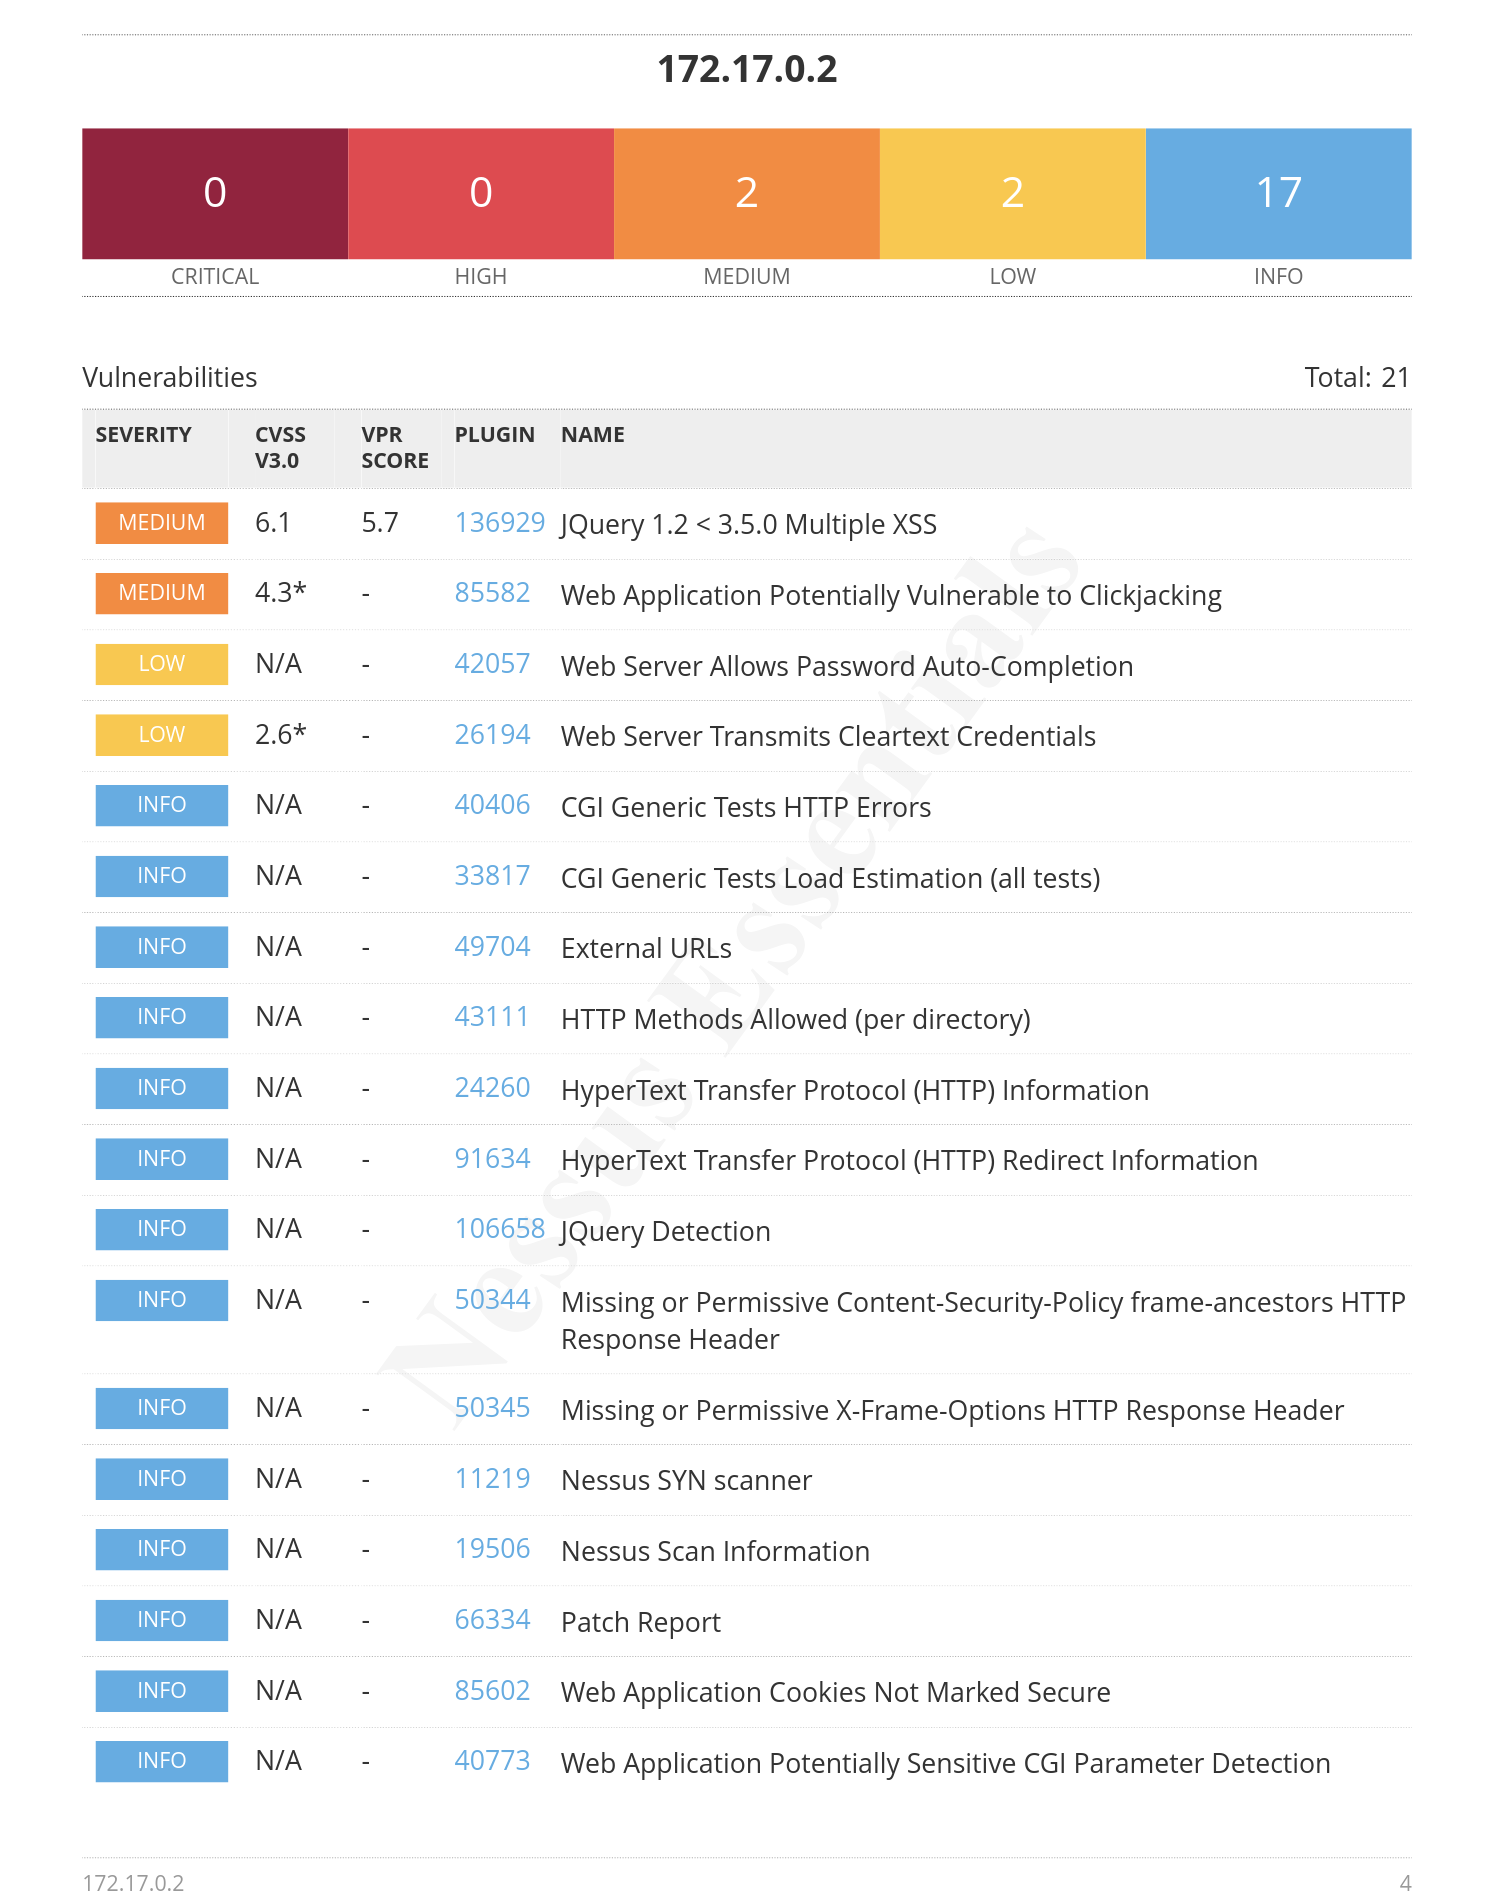
\includegraphics[width=\linewidth]{img/nessus-dvna-before.png}
  \caption{Wyniki skanowania aplikacji DVNA przy użyciu skanera Nessus}
  \label{fig:nessus-dvna-before}
\end{figure}
\begin{figure}[H]
  \centering
  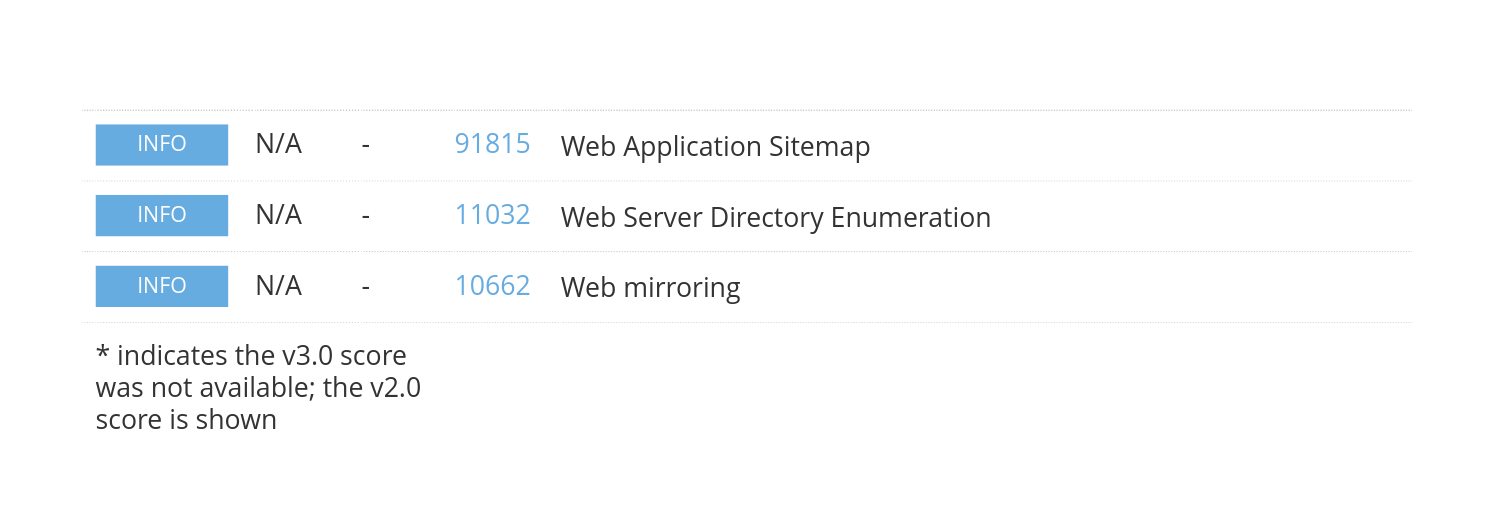
\includegraphics[width=\linewidth]{img/nessus-dvna-before2.png}
  \caption{Wyniki skanowania aplikacji DVNA przy użyciu skanera Nessus}
  \label{fig:nessus-dvna-before2}
\end{figure}

\section{Analiza statyczna i naprawa}

Z wykorzystaniem narzędzia \texttt{gptester} przeprowadzono szczegółową analizę statyczną kodu źródłowego DVNA. Proces ten skupiał się na identyfikacji znanych podatności z listy OWASP Top 10 oraz sugerowaniu możliwych napraw. Po zakończeniu analizy, \texttt{gptester} wygenerował zestaw rekomendacji, które zostały zaimplementowane w kodzie źródłowym aplikacji w celu usunięcia zidentyfikowanych słabości.

\begin{verbatim}
  Found 77 files to scan
  Tokens inside the directory: 22694
\end{verbatim}

\texttt{GPTester} znalazł 77 plików do przeskanowania, zawierających łącznie 22694 tokenów. 

\section{Weryfikacja i ocena skuteczności}

Po wprowadzeniu sugerowanych zmian, aplikacja DVNA została ponownie poddana skanowaniu przy użyciu skanerów OWASP ZAP i Nessus, aby ocenić skuteczność wprowadzonych modyfikacji. Wyniki tego ponownego skanowania zostały porównane z wynikami początkowymi, co pozwoliło na ocenę efektywności narzędzia \texttt{gptester} w kontekście naprawy podatności.

\section{Wyniki i dyskusja}

Analiza wyników wskazała na zauważalną poprawę bezpieczeństwa aplikacji DVNA po zastosowaniu napraw sugerowanych przez \texttt{gptester}. W większości przypadków narzędzie skutecznie zidentyfikowało podatności i zaproponowało adekwatne rozwiązania, które pozytywnie przyczyniły się do zmniejszenia ogólnego ryzyka bezpieczeństwa aplikacji.

\subsection{Wyzwania i ograniczenia}

Jednakże, nie wszystkie sugerowane zmiany były w pełni skuteczne lub odpowiednie dla specyfiki aplikacji DVNA. W niektórych przypadkach, wprowadzenie zmian wymagało dodatkowej analizy i dostosowania sugerowanych rozwiązań do kontekstu aplikacji. Ponadto, niektóre z bardziej złożonych podatności wymagały bardziej zaawansowanych metod naprawczych, co wykraczało poza możliwości automatycznej analizy statycznej.

\section{Wnioski}

Badanie potwierdziło potencjał wykorzystania narzędzia \texttt{gptester} wspieranego przez zaawansowane modele językowe w procesie identyfikacji i naprawy podatności w aplikacjach webowych. Mimo pewnych ograniczeń, narzędzie to stanowi wartościowe wsparcie w procesie zapewniania bezpieczeństwa aplikacji, szczególnie w kontekście szybkiego wykrywania i łagodzenia powszechnych podatności. Dalszy rozwój narzędzia, w tym lepsza integracja z kontekstem aplikacji i zaawansowane metody naprawcze, może znacznie zwiększyć jego skuteczność i przydatność w praktycznych zastosowaniach.

\chapter{Badanie funkcjonalności na aplikacji webowej OWASP VulnerableApp}
\label{sec:badania_na_aplikacji_webowej_owasp}

Analiza funkcjonalności programu do analizy bezpieczeństwa została przeprowadzona z wykorzystaniem aplikacji webowej OWASP VulnerableApp. Jest to narzędzie celowo zawierające liczne podatności, które mają na celu symulację realnych luk bezpieczeństwa, co pozwala na dogłębne testowanie i ocenę narzędzi do skanowania podatności.

\section{Charakterystyka aplikacji OWASP VulnerableApp}
Aplikacja OWASP VulnerableApp została zaprojektowana z myślą o dostarczeniu platformy edukacyjnej dla deweloperów oraz specjalistów od bezpieczeństwa, którzy pragną zgłębić wiedzę na temat bezpieczeństwa aplikacji webowych. Narzędzie to charakteryzuje się skalowalnością, elastycznością oraz łatwością integracji, czyniąc je idealnym środowiskiem do nauki oraz testowania.

\section{Testowane rodzaje podatności}
OWASP VulnerableApp umożliwia testowanie szerokiego zakresu podatności, w tym, ale nie ograniczając się do:
\relax
\begin{itemize}
    \item Podatności JWT
    \item Wstrzykiwanie poleceń (Command Injection)
    \item Podatności związane z przesyłaniem plików (File Upload Vulnerability)
    \item Przejście ścieżki (Path Traversal)
    \item Iniekcje SQL (SQL Injection)
    \item Skrypty międzywitrynowe (XSS)
    \item Ataki oparte na External XML Entities (XXE)
    \item Open Redirect
    \item Server-Side Request Forgery (SSRF)
\end{itemize}

Zawarte podatności są reprezentatywne dla typowych zagrożeń w aplikacjach internetowych, co pozwala na wszechstronne i realistyczne testowanie narzędzi do ich wykrywania i naprawy.

\section{Zawartość znajdująca się w repozytorium}
Repozytorium aplikacji VulnerableApp zawiera projekt aplikacji webowej napisany w następującym stosie technologicznym:
\begin{itemize}
    \item Java 8
    \item Spring Boot
    \item Maven 3.6.1
    \item ReactJS
    \item Javascript/TypeScript
\end{itemize} 

\begin{verbatim}
 > ./main.py ../testing-envs/VulnerableApp/

                  ___  ___  _____           _             
                 / __|| _ \|_   _| ___  ___| |_  ___  _ _ 
                | (_ ||  _/  | |  / -_)(_-/|  _|/ -_)| '_|
                 \___||_|    |_|  \___|/__/ \__|\___||_|  

           The static code analysis agent, version: assistant-0.3


2024-01-25 22:05:23: Beginning scan for ../testing-envs/VulnerableApp/
2024-01-25 22:05:23: Found 97 files to scan
2024-01-25 22:05:23: Tokens inside the directory: 77513
2024-01-25 22:05:23: Using model: gpt-4-1106-preview
2024-01-25 22:05:23: Beginning code analysis...
\end{verbatim}

W repozytorium znajduje się 231 plików, które zawierają 229119 tokenów z uwzględnieniem wszystkich plików. Nasz program pokazał wartości dla plików zawierających kod, a dokładnie tych które nie są wyspecjalizowane w liście nazw do ignorowania.

\section{Procedura przeprowadzenia testów}
Testy zostały przeprowadzone przy użyciu najnowszej wersji programu, zgodnie z następującymi krokami:

\begin{enumerate}
    \item Przygotowanie środowiska testowego z wykorzystaniem aplikacji OWASP VulnerableApp.
    \item Uruchomienie skanowania z wykorzystaniem programu.
    \item Dokumentacja wykrytych podatności oraz sugerowanych przez program napraw.
    \item Analiza efektywności napraw i ich wpływ na bezpieczeństwo aplikacji za pomocą innych skanerów podatności.
\end{enumerate}

\subsection{Oczekiwane rezultaty}
W wyniku przeprowadzonych testów oczekujemy uzyskania szczegółowych danych na temat liczby wykrytych podatności, rodzajów podatności, a także czasu potrzebnego na ich wykrycie i naprawę. Dane te zostaną następnie wykorzystane do stworzenia szczegółowych wykresów i tabel ilustrujących skuteczność programu.

\section{Wnioski i dalsze kierunki badań}
Na podstawie zebranych danych zostaną wyciągnięte wnioski dotyczące skuteczności narzędzia w kontekście poszczególnych typów podatności oraz ogólnej wydajności. Dalsze badania mogą również koncentrować się na porównaniu wyników z innymi narzędziami dostępnymi na rynku oraz na rozwoju nowych funkcji i usprawnień w badanym programie.

\chapter{Przeprowadzenie testów na aplikacji NodeGoat}

\section{Wstęp}
\label{sec:wstep}
\dots

\section{Przygotowanie środowiska testowego}
\label{sec:przygotowanie_srodowiska_testowego}

Aby przygotować aplikację do lokalnego uruchomienia bez korzystania z konteneryzacji, niezbędne było poprawienie wersji paczek w pliku package.json oraz obniżenie używanej wersji npm i node do node v16.0.0 (npm v7.10.0). Następnie należało zainstalować wszystkie zależności za pomocą komendy npm install. Po wykonaniu tych kroków aplikacja była gotowa do uruchomienia komendą npm run.

\section{Testy funkcjonalne przed zmianami}
\label{sec:testy_funkcjonalne_przed_zmianami}

\begin{figure}[H]
  \centering
  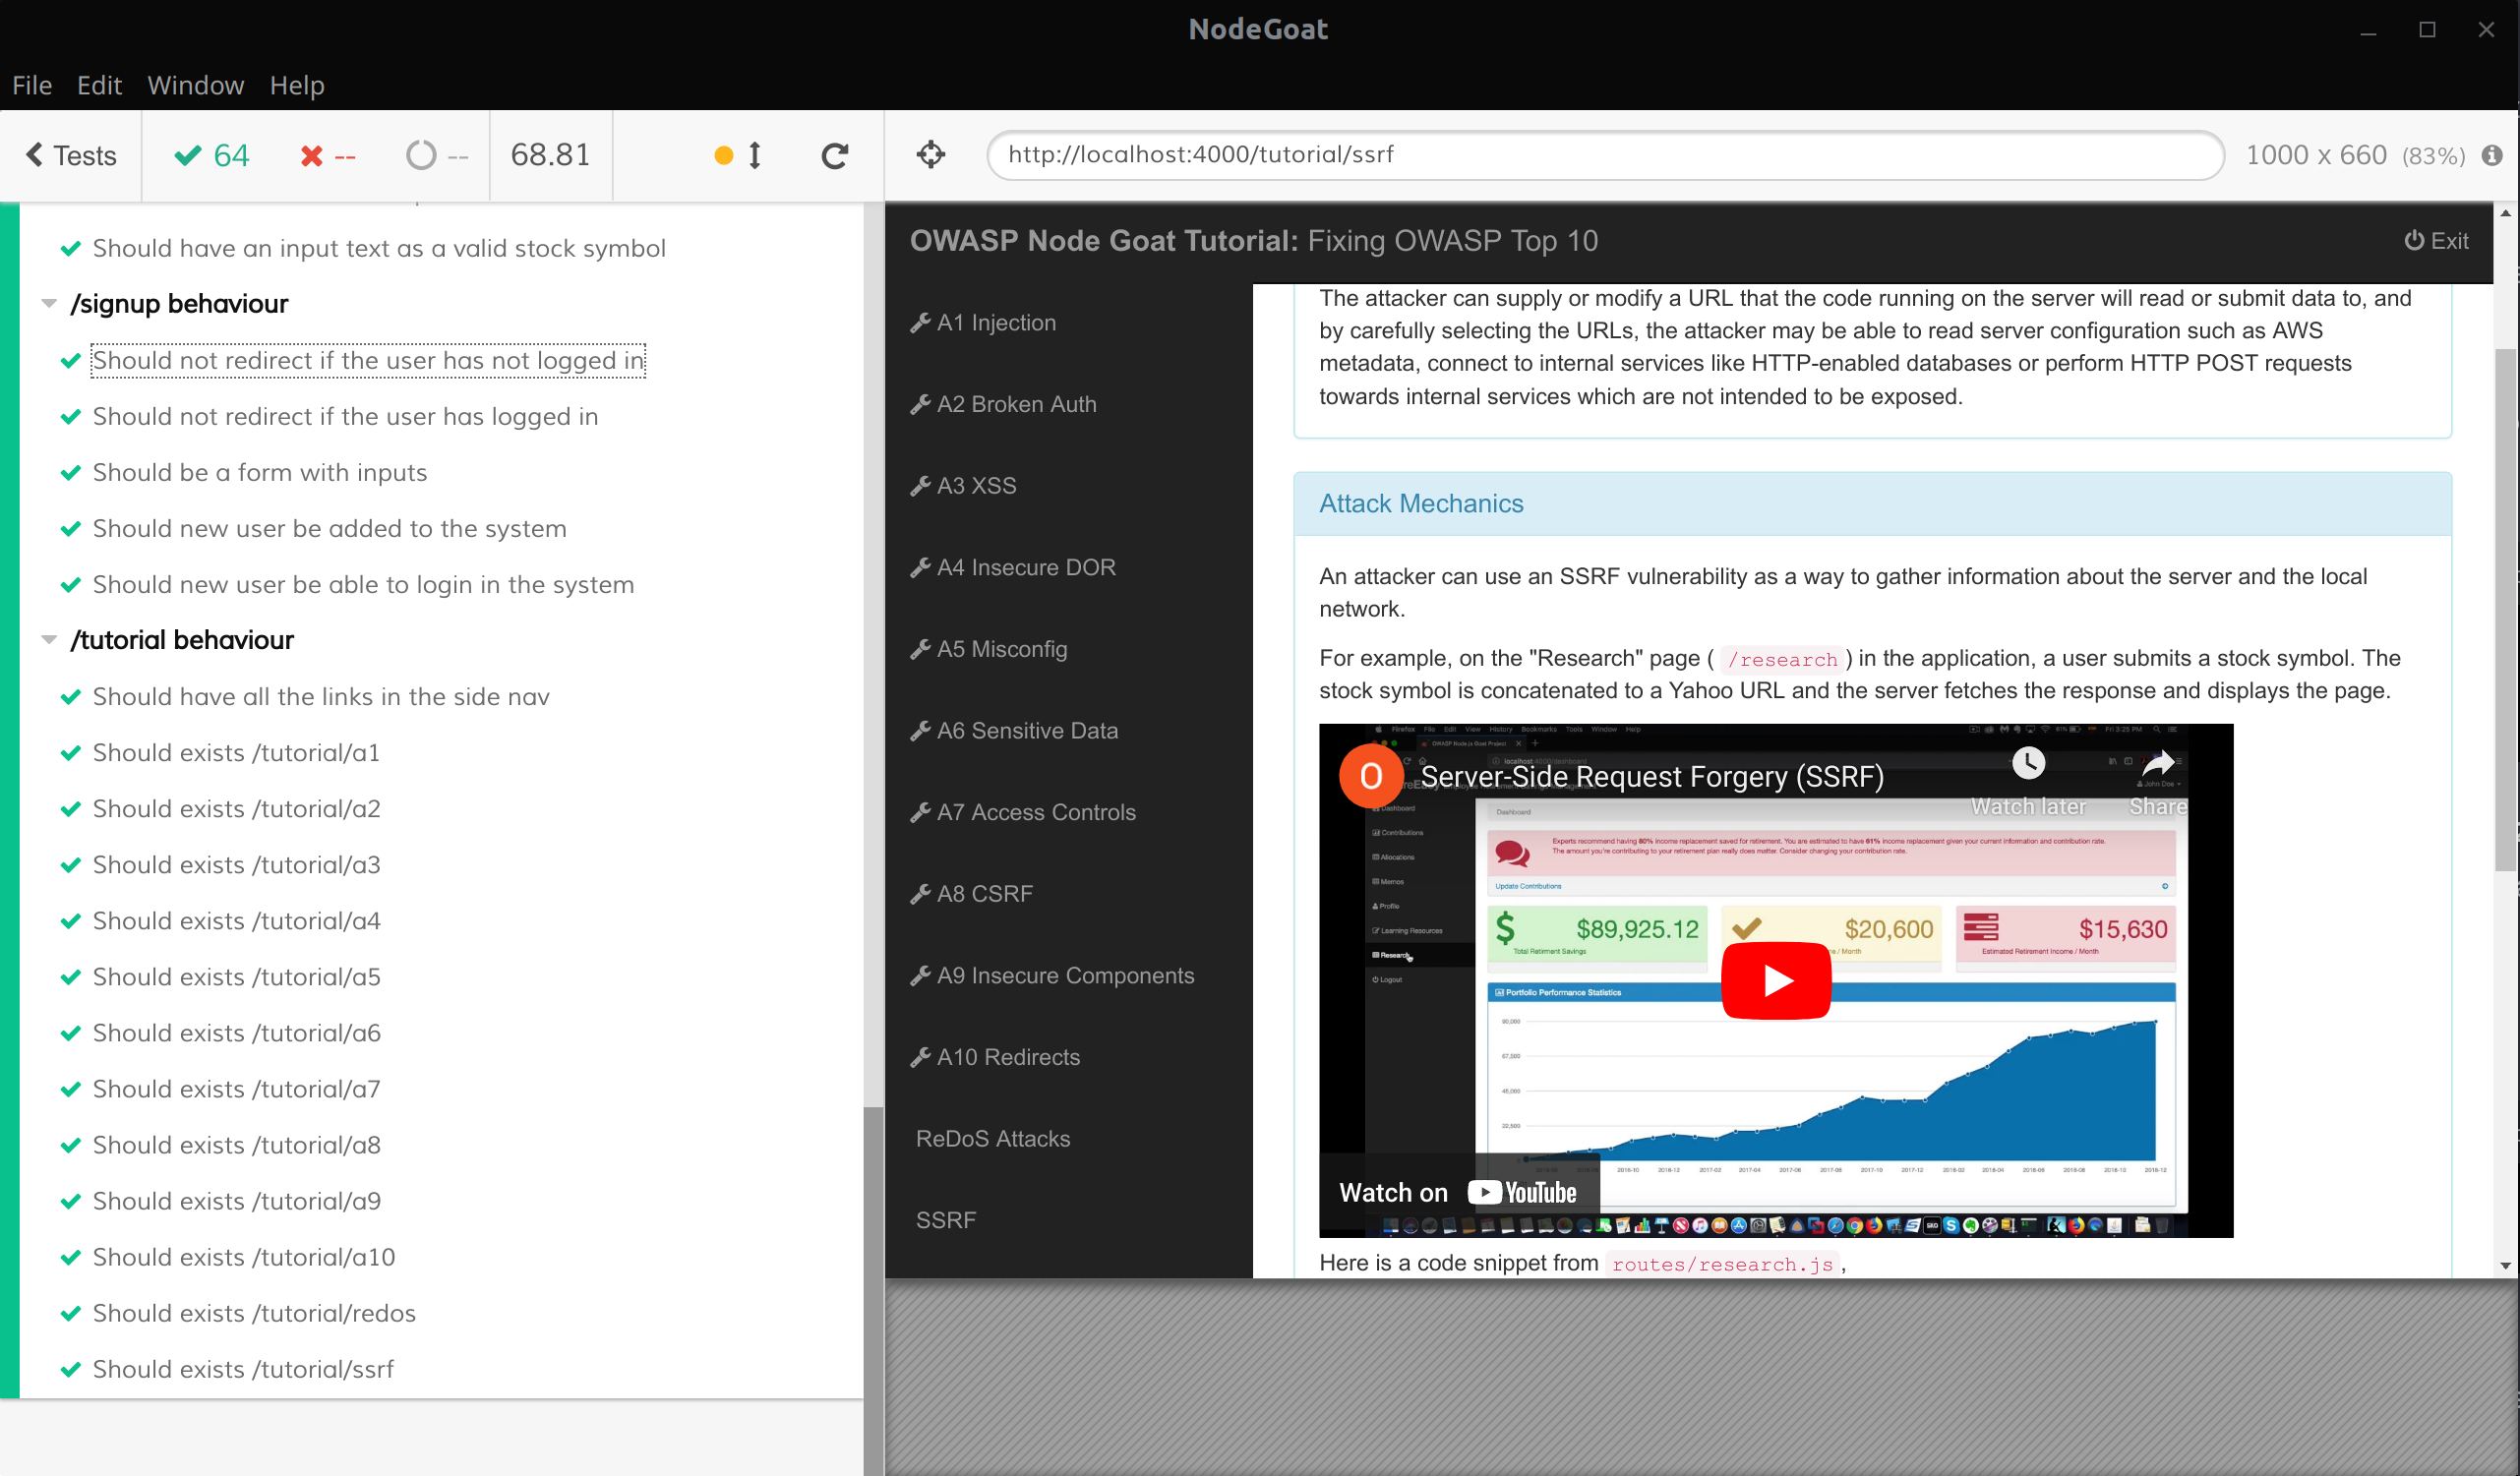
\includegraphics[width=\linewidth]{img/func-test-goat-before.png}
  \caption{Wyniki testów funkcjonalnych aplikacji NodeGoat przed wprowadzeniem zmian}
  \label{fig:nodegoat-before}
\end{figure}

\section{Identyfikacja podatności za pomocą tradycyjnych skanerów}
Przed przystąpieniem do naprawy podatności, aplikacja DVNA została poddana skanowaniu przy użyciu skanerów OWASP ZAP i Nessus. Wyniki tych skanowań zostały wykorzystane jako punkt odniesienia do oceny skuteczności narzędzia \texttt{gptester} w kontekście naprawy podatności.


\subsection{OWASP ZAP}
\label{subsec:owasp_zap}
Skanowanie aplikacji NodeGoat przy użyciu OWASP ZAP wykazało obecność 20 podatności, w tym 3 krytyczne, 5 wysokiego ryzyka, 5 średniego ryzyka oraz 7 niskiego ryzyka. Poniżej przedstawiono listę zidentyfikowanych podatności wraz z ich ryzykiem i opisem.

\begin{table}[H]
  \caption{Wyniki skanowania aplikacji NodeGoat przy użyciu skanera \texttt{OWASP-zap}}
  \begin{tabular}{llllll}
    \multicolumn{2}{l}{} &
      \multicolumn{4}{c}{Risk} \\ \cline{3-6} 
    \multicolumn{2}{l|}{} &
      \multicolumn{1}{l|}{\begin{tabular}[c]{@{}l@{}}High\\ (= High)\end{tabular}} &
      \multicolumn{1}{l|}{\begin{tabular}[c]{@{}l@{}}Medium\\ (\textgreater{}= Medium)\end{tabular}} &
      \multicolumn{1}{l|}{\begin{tabular}[c]{@{}l@{}}Low\\ (\textgreater{}= Low)\end{tabular}} &
      \multicolumn{1}{l|}{\begin{tabular}[c]{@{}l@{}}Informational\\ (\textgreater{}= Informational)\end{tabular}} \\ \cline{2-6} 
    \multicolumn{1}{l|}{site} &
      \multicolumn{1}{l|}{http://localhost:4000} &
      \multicolumn{1}{l|}{\begin{tabular}[c]{@{}l@{}}3\\ (3)\end{tabular}} &
      \multicolumn{1}{l|}{\begin{tabular}[c]{@{}l@{}}5\\ (8)\end{tabular}} &
      \multicolumn{1}{l|}{\begin{tabular}[c]{@{}l@{}}5\\ (13)\end{tabular}} &
      \multicolumn{1}{l|}{\begin{tabular}[c]{@{}l@{}}7\\ (20)\end{tabular}} \\ \cline{2-6} 
    \end{tabular}   
  \label{tab:zap_before}
  \end{table}

  \begin{table}[htbp]
    \centering
    \scriptsize
    \caption{Podsumowanie typów alertów i powiązanych zagrożeń}
    \label{tab:alert_summary}
    \begin{tabular}{|l|l|r|}
    \hline
    \textbf{Alert Type} & \textbf{Risk} & \textbf{Count (\%)} \\
    \hline
    Cross Site Scripting (Reflected) & High & 3 (15.0\%) \\
    External Redirect & High & 1 (5.0\%) \\
    Open Redirect & High & 1 (5.0\%) \\
    CSP: Wildcard Directive & Medium & 16 (80.0\%) \\
    Content Security Policy (CSP) Header Not Set & Medium & 24 (120.0\%) \\
    Directory Browsing & Medium & 2 (10.0\%) \\
    Missing Anti-clickjacking Header & Medium & 24 (120.0\%) \\
    Vulnerable JS Library & Medium & 2 (10.0\%) \\
    Cookie without SameSite Attribute & Low & 5 (25.0\%) \\
    Cross-Domain JavaScript Source File Inclusion & Low & 24 (120.0\%) \\
    Server Leaks Information via "X-Powered-By" HTTP Response Header Field(s) & Low & 63 (315.0\%) \\
    Timestamp Disclosure - Unix & Low & 1 (5.0\%) \\
    X-Content-Type-Options Header Missing & Low & 37 (185.0\%) \\
    Authentication Request Identified & Informational & 1 (5.0\%) \\
    Information Disclosure - Suspicious Comments & Informational & 26 (130.0\%) \\
    Loosely Scoped Cookie & Informational & 5 (25.0\%) \\
    Modern Web Application & Informational & 23 (115.0\%) \\
    Session Management Response Identified & Informational & 8 (40.0\%) \\
    User Agent Fuzzer & Informational & 290 (1,450.0\%) \\
    User Controllable HTML Element Attribute (Potential XSS) & Informational & 2 (10.0\%) \\
    \hline
    \textbf{Total} & & \textbf{Various} \\
    \hline
    \end{tabular}
    \end{table}
    

\subsection{Nessus}
\label{subsec:nessus}
Skanowanie aplikacji DVNA przy użyciu Nessus wykazało obecność 21 podatności, w tym 2 średniego ryzyka, 2 niskiego ryzyka oraz 17 informacyjnych. Poniżej przedstawiono listę zidentyfikowanych podatności wraz z ich ryzykiem i opisem.


\subsection{Statyczny analizator CodeQL}\label{subsec:codeql}

\subsubsection{Proces przeprowadzenia testu}

\begin{enumerate}
    \item Przygotowanie środowiska testowego dla aplikacji NodeGoat.
    
    

    \item Uruchomienie skanowania z wykorzystaniem programu.
    Przed przystąpieniem do skanowania należy utworzyć bazę danych CodeQL. W tym celu należy wykonać następujące kroki:
    \begin{enumerate}
        \item Zainstalować CodeQL CLI.
        \item Zainicjalizować i zbudować bazę danych CodeQL.
        \begin{verbatim}
        > codeql database create GoatQL-db --language=javascript  
        Initializing database at /home/paris/projekty/INZYNIERKA/testing-envs/NodeGoat/GoatQL-db.
        Running build command: []
        [2024-01-25 19:33:30] [build-stdout] Single-threaded extraction.
        [2024-01-25 19:33:34] [build-stdout] package.json: Main file set to server.js
        [2024-01-25 19:33:34] [build-stdout] Extracting /home/paris/projekty/INZYNIERKA/testing-envs/NodeGoat/app/views/tutorial/a1.html
        [2024-01-25 19:33:34] [build-stdout] Done extracting /home/paris/projekty/INZYNIERKA/testing-envs/NodeGoat/app/views/tutorial/a1.html (91 ms)
        [2024-01-25 19:33:34] [build-stdout] Extracting /home/paris/projekty/INZYNIERKA/testing-envs/NodeGoat/app/views/tutorial/a10.html
        [2024-01-25 19:33:34] [build-stdout] Done extracting /home/paris/projekty/INZYNIERKA/testing-envs/NodeGoat/app/views/tutorial/a10.html (5 ms)
        [2024-01-25 19:33:34] [build-stdout] Extracting /home/paris/projekty/INZYNIERKA/testing-envs/NodeGoat/app/views/tutorial/a2.html
        .
        .
        .
        [2024-01-30 19:33:38] [build-stdout] Extracting /home/paris/Downloads/tar/codeql-bundle-linux64/codeql/javascript/tools/data/externs/nodejs/vm.js
        [2024-01-30 19:33:38] [build-stdout] Done extracting /home/paris/Downloads/tar/codeql-bundle-linux64/codeql/javascript/tools/data/externs/nodejs/vm.js (8 ms)
        Finalizing database at /home/paris/projekty/INZYNIERKA/testing-envs/NodeGoat/GoatQL-db.
        Successfully created database at /home/paris/projekty/INZYNIERKA/testing-envs/NodeGoat/GoatQL-db.
        \end{verbatim}

        \item Uruchomić wybrane zapytania na bazie danych wyszukujące podatności.
        
        W tym celu uruchomiłem domyślne pakiety zapytań dostępne w CodeQL CLI. W celu uruchomienia zapytania należy wykonać następującą komendę:
        \begin{verbatim}
          > codeql database analyze GoatQL-db javascript-code-scanning.qls --format=csv --output=default-goat-QLresults.csv
Running queries.
[1/88] Loaded /home/paris/Downloads/tar/codeql-bundle-linux64/codeql/qlpacks/codeql/javascript-queries/0.8.2/AngularJS/InsecureUrlWhitelist.qlx.
        \end{verbatim}
        Komenda zakończyła się sukcesem, a w katalogu pojawił się plik z wynikami analizy.
        \begin{verbatim}
          PrototypePollutingFunction.ql            : [83/88 eval 25ms] Results written to codeql/javascript-queri
PrototypePollutingMergeCall.ql           : [84/88 eval 260ms] Results written to codeql/javascript-quer
InsufficientPasswordHash.ql              : [85/88 eval 5ms] Results written to codeql/javascript-querie
RequestForgery.ql                        : [86/88 eval 143ms] Results written to codeql/javascript-quer
LinesOfCode.ql                           : [87/88 eval 3ms] Results written to codeql/javascript-querie
LinesOfUserCode.ql                       : [88/88 eval 644ms] Results written to codeql/javascript-quer
Shutting down query evaluator.
Interpreting results.
Analysis produced the following diagnostic data:

|          Diagnostic          |  Summary   |
+------------------------------+------------+
| Successfully extracted files | 77 results |

Analysis produced the following metric data:

|                                   Metric                                   | Value |
+----------------------------------------------------------------------------+-------+
| Total lines of user written JavaScript and TypeScript code in the database |  2926 |
| Total lines of JavaScript and TypeScript code in the database              |  2932 |
\end{verbatim}

Na aplikacji został również uruchomiony pakiet kwerend javascript-extended-security.qls 
    \end{enumerate}

    \item Dokumentacja wykrytych podatności oraz sugerowanych przez program napraw.
    \item Analiza efektywności napraw i ich wpływ na bezpieczeństwo aplikacji za pomocą innych skanerów podatności.
\end{enumerate}

\subsection{Wyniki otrzymane z analizy CodeQL}
\begin{table}[H]
  \centering
  \footnotesize
  % \resizebox{\textwidth}{!}{%
  \begin{tabular}{|l|l|l|l|l|l|l|l|l|l|}
  \hline
      "Inefficient regular expression" & "A regular expression that requires exponential time to match certain inputs can be a performance bottleneck, and may be vulnerable to denial-of-service attacks." & "error" & "This part of the regular expression may cause exponential backtracking on strings containing many repetitions of '0'." & "/app/routes/profile.js" & "59" & "32" & "59" & "37" & ~ \\ \hline
      "Polynomial regular expression used on uncontrolled data" & "A regular expression that can require polynomial time to match may be vulnerable to denial-of-service attacks." & "warning" & "This [[""regular expression""|""relative:///app/routes/profile.js:59:32:59:37""]] that depends on [[""a user-provided value""|""relative:///app/routes/profile.js:50:13:50:20""]] may run slow on strings with many repetitions of '0'." & "/app/routes/profile.js" & "61" & "44" & "61" & "73" & ~ \\ \hline
      "Polynomial regular expression used on uncontrolled data" & "A regular expression that can require polynomial time to match may be vulnerable to denial-of-service attacks." & "warning" & "This [[""regular expression""|""relative:///app/routes/session.js:143:34:143:38""]] that depends on [[""a user-provided value""|""relative:///app/routes/session.js:198:13:198:20""]] may run slow on strings starting with '$\backslash$t@' and with many repetitions of '$\backslash$t@'. & ~ & ~ & ~ & ~ & ~ & ~ \\ \hline
      This [[""regular expression""|""relative:///app/routes/session.js:143:41:143:45""]] that depends on [[""a user-provided value""|""relative:///app/routes/session.js:198:13:198:20""]] may run slow on strings starting with '$\backslash$t@$\backslash$t.' and with many repetitions of '$\backslash$t.'." & "/app/routes/session.js" & "181" & "18" & "181" & "37" & ~ & ~ & ~ & ~ \\ \hline
      "Database query built from user-controlled sources" & "Building a database query from user-controlled sources is vulnerable to insertion of malicious code by the user." & "error" & "This query object depends on a [[""user-provided value""|""relative:///app/routes/session.js:57:13:57:20""]]." & "/app/data/user-dao.js" & "91" & "26" & "93" & "9" & ~ \\ \hline
      "Database query built from user-controlled sources" & "Building a database query from user-controlled sources is vulnerable to insertion of malicious code by the user." & "error" & "This query object depends on a [[""user-provided value""|""relative:///app/routes/session.js:198:13:198:20""]]." & "/app/data/user-dao.js" & "104" & "26" & "106" & "9" & ~ \\ \hline
      "Clear text transmission of sensitive cookie" & "Sending sensitive information in a cookie without requring SSL encryption can expose the cookie to an attacker." & "warning" & "Sensitive cookie sent without enforcing SSL encryption." & "/server.js" & "78" & "13" & "102" & "6" & ~ \\ \hline
      "Missing CSRF middleware" & "Using cookies without CSRF protection may allow malicious websites to submit requests on behalf of the user." & "error" & "This cookie middleware is serving a [[""request handler""|""relative:///app/routes/index.js:34:24:34:56""]] without CSRF protection. & ~ & ~ & ~ & ~ & ~ & ~ \\ \hline
      This cookie middleware is serving a [[""request handler""|""relative:///app/routes/index.js:38:25:38:51""]] without CSRF protection. & ~ & ~ & ~ & ~ & ~ & ~ & ~ & ~ & ~ \\ \hline
      This cookie middleware is serving a [[""request handler""|""relative:///app/routes/index.js:48:26:48:35""]] without CSRF protection. & ~ & ~ & ~ & ~ & ~ & ~ & ~ & ~ & ~ \\ \hline
      This cookie middleware is serving a [[""request handler""|""relative:///app/routes/index.js:48:38:48:71""]] without CSRF protection. & ~ & ~ & ~ & ~ & ~ & ~ & ~ & ~ & ~ \\ \hline
      This cookie middleware is serving a [[""request handler""|""relative:///app/routes/index.js:52:32:52:41""]] without CSRF protection. & ~ & ~ & ~ & ~ & ~ & ~ & ~ & ~ & ~ \\ \hline
      This cookie middleware is serving a [[""request handler""|""relative:///app/routes/index.js:52:44:52:89""]] without CSRF protection. & ~ & ~ & ~ & ~ & ~ & ~ & ~ & ~ & ~ \\ \hline
      This cookie middleware is serving a [[""request handler""|""relative:///app/routes/index.js:56:27:56:36""]] without CSRF protection. & ~ & ~ & ~ & ~ & ~ & ~ & ~ & ~ & ~ \\ \hline
      This cookie middleware is serving a [[""request handler""|""relative:///app/routes/index.js:67:24:67:33""]] without CSRF protection. & ~ & ~ & ~ & ~ & ~ & ~ & ~ & ~ & ~ \\ \hline
      This cookie middleware is serving a [[""request handler""|""relative:///app/routes/index.js:67:36:67:56""]] without CSRF protection." & "/server.js" & "78" & "13" & "102" & "6" & ~ & ~ & ~ & ~ \\ \hline
      "Server-side URL redirect" & "Server-side URL redirection based on unvalidated user input may cause redirection to malicious web sites." & "warning" & "Untrusted URL redirection depends on a [[""user-provided value""|""relative:///app/routes/index.js:72:29:72:41""]]." & "/app/routes/index.js" & "72" & "29" & "72" & "41" & ~ \\ \hline
      "Code injection" & "Interpreting unsanitized user input as code allows a malicious user arbitrary code execution." & "error" & "This code execution depends on a [[""user-provided value""|""relative:///app/routes/allocations.js:20:13:20:21""]]." & "/app/data/allocations-dao.js" & "78" & "29" & "78" & "92" & ~ \\ \hline
      "Code injection" & "Interpreting unsanitized user input as code allows a malicious user arbitrary code execution." & "error" & "This code execution depends on a [[""user-provided value""|""relative:///app/routes/contributions.js:32:29:32:36""]]." & "/app/routes/contributions.js" & "32" & "29" & "32" & "43" & ~ \\ \hline
      "Code injection" & "Interpreting unsanitized user input as code allows a malicious user arbitrary code execution." & "error" & "This code execution depends on a [[""user-provided value""|""relative:///app/routes/contributions.js:33:31:33:38""]]." & "/app/routes/contributions.js" & "33" & "31" & "33" & "47" & ~ \\ \hline
      "Code injection" & "Interpreting unsanitized user input as code allows a malicious user arbitrary code execution." & "error" & "This code execution depends on a [[""user-provided value""|""relative:///app/routes/contributions.js:34:27:34:34""]]." & "/app/routes/contributions.js" & "34" & "27" & "34" & "39" & ~ \\ \hline
      "Missing rate limiting" & "An HTTP request handler that performs expensive operations without restricting the rate at which operations can be carried out is vulnerable to denial-of-service attacks." & "warning" & "This route handler performs [[""authorization""|""relative:///app/routes/session.js:58:9:118:10""]] & but is not rate-limited." & "/app/routes/index.js" & "34" & "24" & "34" & "56" \\ \hline
      "Server-side request forgery" & "Making a network request with user-controlled data in the URL allows for request forgery attacks." & "error" & "The [[""URL""|""relative:///app/routes/research.js:16:31:16:33""]] of this request depends on a [[""user-provided value""|""relative:///app/routes/research.js:15:25:15:37""]]." & "/app/routes/research.js" & "16" & "20" & "28" & "14" & ~ \\ \hline
      "DOM text reinterpreted as HTML" & "Reinterpreting text from the DOM as HTML can lead to a cross-site scripting vulnerability." & "warning" & "[[""DOM text""|""relative:///app/assets/vendor/bootstrap/bootstrap.js:11:200:11:220""]] is reinterpreted as HTML without escaping meta-characters." & "/app/assets/vendor/bootstrap/bootstrap.js" & "11" & "288" & "11" & "288" & ~ \\ \hline
      "DOM text reinterpreted as HTML" & "Reinterpreting text from the DOM as HTML can lead to a cross-site scripting vulnerability." & "warning" & "[[""DOM text""|""relative:///app/assets/vendor/bootstrap/bootstrap.js:11:5190:11:5210""]] is reinterpreted as HTML without escaping meta-characters." & "/app/assets/vendor/bootstrap/bootstrap.js" & "11" & "5190" & "11" & "5262" & ~ \\ \hline
      "DOM text reinterpreted as HTML" & "Reinterpreting text from the DOM as HTML can lead to a cross-site scripting vulnerability." & "warning" & "[[""DOM text""|""relative:///app/assets/vendor/bootstrap/bootstrap.js:11:5822:11:5842""]] is reinterpreted as HTML without escaping meta-characters." & "/app/assets/vendor/bootstrap/bootstrap.js" & "11" & "5926" & "11" & "5926" & ~ \\ \hline
      "DOM text reinterpreted as HTML" & "Reinterpreting text from the DOM as HTML can lead to a cross-site scripting vulnerability." & "warning" & "[[""DOM text""|""relative:///app/assets/vendor/bootstrap/bootstrap.js:11:10957:11:10977""]] is reinterpreted as HTML without escaping meta-characters." & "/app/assets/vendor/bootstrap/bootstrap.js" & "11" & "10957" & "11" & "11012" & ~ \\ \hline
      "DOM text reinterpreted as HTML" & "Reinterpreting text from the DOM as HTML can lead to a cross-site scripting vulnerability." & "warning" & "[[""DOM text""|""relative:///app/assets/vendor/bootstrap/bootstrap.js:11:16632:11:16660""]] is reinterpreted as HTML without escaping meta-characters." & "/app/assets/vendor/bootstrap/bootstrap.js" & "11" & "15401" & "11" & "15401" & ~ \\ \hline
      "DOM text reinterpreted as HTML" & "Reinterpreting text from the DOM as HTML can lead to a cross-site scripting vulnerability." & "warning" & "[[""DOM text""|""relative:///app/assets/vendor/bootstrap/bootstrap.js:11:19467:11:19487""]] is reinterpreted as HTML without escaping meta-characters." & "/app/assets/vendor/bootstrap/bootstrap.js" & "11" & "19722" & "11" & "19722" & ~ \\ \hline
      "DOM text reinterpreted as HTML" & "Reinterpreting text from the DOM as HTML can lead to a cross-site scripting vulnerability." & "warning" & "[[""DOM text""|""relative:///app/assets/vendor/bootstrap/bootstrap.js:11:24674:11:24694""]] is reinterpreted as HTML without escaping meta-characters." & "/app/assets/vendor/bootstrap/bootstrap.js" & "11" & "24772" & "11" & "24772" & ~ \\ \hline
      "DOM text reinterpreted as HTML" & "Reinterpreting text from the DOM as HTML can lead to a cross-site scripting vulnerability." & "warning" & "[[""DOM text""|""relative:///app/assets/vendor/bootstrap/bootstrap.js:11:24823:11:24843""]] is reinterpreted as HTML without escaping meta-characters." & "/app/assets/vendor/bootstrap/bootstrap.js" & "11" & "24852" & "11" & "24852" & ~ \\ \hline
      "Unsafe jQuery plugin" & "A jQuery plugin that unintentionally constructs HTML from some of its options may be unsafe to use for clients." & "warning" & "Potential XSS vulnerability in the [[""'\$.fn.tooltip' plugin""|""relative:///app/assets/vendor/bootstrap/bootstrap.js:11:17473:11:17642""]]." & "/app/assets/vendor/bootstrap/bootstrap.js" & "11" & "13968" & "11" & "13989" & ~ \\ \hline
      "Unsafe jQuery plugin" & "A jQuery plugin that unintentionally constructs HTML from some of its options may be unsafe to use for clients." & "warning" & "Potential XSS vulnerability in the [[""'\$.fn.collapse' plugin""|""relative:///app/assets/vendor/bootstrap/bootstrap.js:11:24276:11:24480""]]." & "/app/assets/vendor/bootstrap/bootstrap.js" & "11" & "22543" & "11" & "22561" & ~ \\ \hline
      "Unsafe jQuery plugin" & "A jQuery plugin that unintentionally constructs HTML from some of its options may be unsafe to use for clients." & "warning" & "Potential XSS vulnerability in the [[""'\$.fn.scrollspy' plugin""|""relative:///app/assets/vendor/bootstrap/bootstrap.js:11:26745:11:26918""]]." & "/app/assets/vendor/bootstrap/bootstrap.js" & "11" & "26431" & "11" & "26443" & ~ \\ \hline
      "Unsafe jQuery plugin" & "A jQuery plugin that unintentionally constructs HTML from some of its options may be unsafe to use for clients." & "warning" & "Potential XSS vulnerability in the [[""'\$.fn.scrollspy' plugin""|""relative:///app/assets/vendor/bootstrap/bootstrap.js:11:26745:11:26918""]]." & "/app/assets/vendor/bootstrap/bootstrap.js" & "11" & "26567" & "11" & "26567" & ~ \\ \hline
  \end{tabular}
\end{table}
Rozszerzony pakiet kwerend rozszerzył wyniki o następujące wpisy:

\begin{table}[!ht]
  \centering
  \resizebox{\textwidth}{!}{%
  \begin{tabular}{|l|l|l|l|l|l|l|l|}
    \hline
    \textbf{Issue} & \textbf{Description} & \textbf{Severity} & \textbf{Details} & \textbf{File} & \textbf{Start Line} & \textbf{Start Column} & \textbf{End Line} & \textbf{End Column} \\ \hline
    "Failure to abandon session" & "Reusing an existing session as a different user could allow an attacker to access someone else's account by using their session." & "warning" & "Route handler does not invalidate session following login." & "/app/routes/index.js" & "34" & "5" & "34" & "57" \\ \hline
    "Log injection" & "Building log entries from user-controlled sources is vulnerable to insertion of forged log entries by a malicious user." & "error" & "Log entry depends on a [[""user-provided value""|""relative:///app/routes/session.js:57:13:57:20""]]." & "/app/routes/session.js" & "64" & "80" & "64" & "87" \\ \hline
    "Indirect uncontrolled command line" & "Forwarding command-line arguments to a child process executed within a shell may indirectly introduce command-line injection vulnerabilities." & "warning" & "This command depends on an unsanitized [[""environment variable""|""relative:///Gruntfile.js:159:24:159:34""]]." & "/Gruntfile.js" & "166" & "13" & "166" & "46" \\ \hline
  \end{tabular}}
  \caption{Rozszerzone wyniki skanowania aplikacji NodeGoat przy użyciu skanera \texttt{CodeQL}}
\end{table}


\section{Analiza GPTester z wykorzsytaniem RAG}
Z uwagi na wielkość projektu i limit dla API asystentów wynoszący 32768 znaków (nie tokenów), kod był przetwarzany przez aplikację w aż 50 częściach asynchronicznie. Wykorzystana została dodatkowo funkcja generacji wspomaganej pobieraniem danych. 

Niestety firmowy klucz API OpenAI, z którego korzystałem by wykonać skan został pod sam koniec wycofany, prawdopobnie przez dużą liczbę zapytań. W związku z tym, udało się przeprowadzić skanowanie tylko dla ~45 części kodu, co stanowiło około 9/10 kodu aplikacji. Skanowanych było o 10 plików więcej niż uwzględniał CodeQL, co wynikało z faktu, że CodeQL nie uwzględniał plików konfiguracyjnych i tych z rozszerzeniem .ejs, które zawierały kod HTML.
Pozwoliło to agentowi na aktualizację wersji oprogramowania
\section{Analiza GPTester bez RAG}
Następnie uruchomiłem proces analizy kodu za pomocą GPTester bez użycia RAG. W tym celu wykorzystałem prywatny klucz API OpenAI, dzięki czemu mogłem dowiedzieć się jakie koszty są generowane podczas skanowania. 

\section{Wnioski}
\label{sec:wnioski}

Na podstawie przeprowadzonych badań eksperymentalnych udało się zweryfikować założenia dotyczące efektywności wykorzystania modeli AI w procesie identyfikacji i naprawy podatności w kodzie źródłowym. Główne wnioski to:

% Tutaj należy wstawić wnioski z badania